\section{Simulation Analysis}
\label{sec:simulation}


	In order to run the simulation, we wrote the ngspice code according to the image below. It is important to note that an extra voltage source, Vaux, was added and therefore, another node was also added (node 8). This Vaux was intended to allow the measurement of the current Ic which voltage source Vc depends on, since ngspice doesn't allow us to introduce Resistor R6's current in the computation. Vaux's voltage is equal to 0 V, since it is only an auxiliary component that doesn't interfere with the circuit (node's 8 voltage is equal to node's 7 voltage) and allowed us to obtain the current through it.

\begin{figure}[ht]
\centering
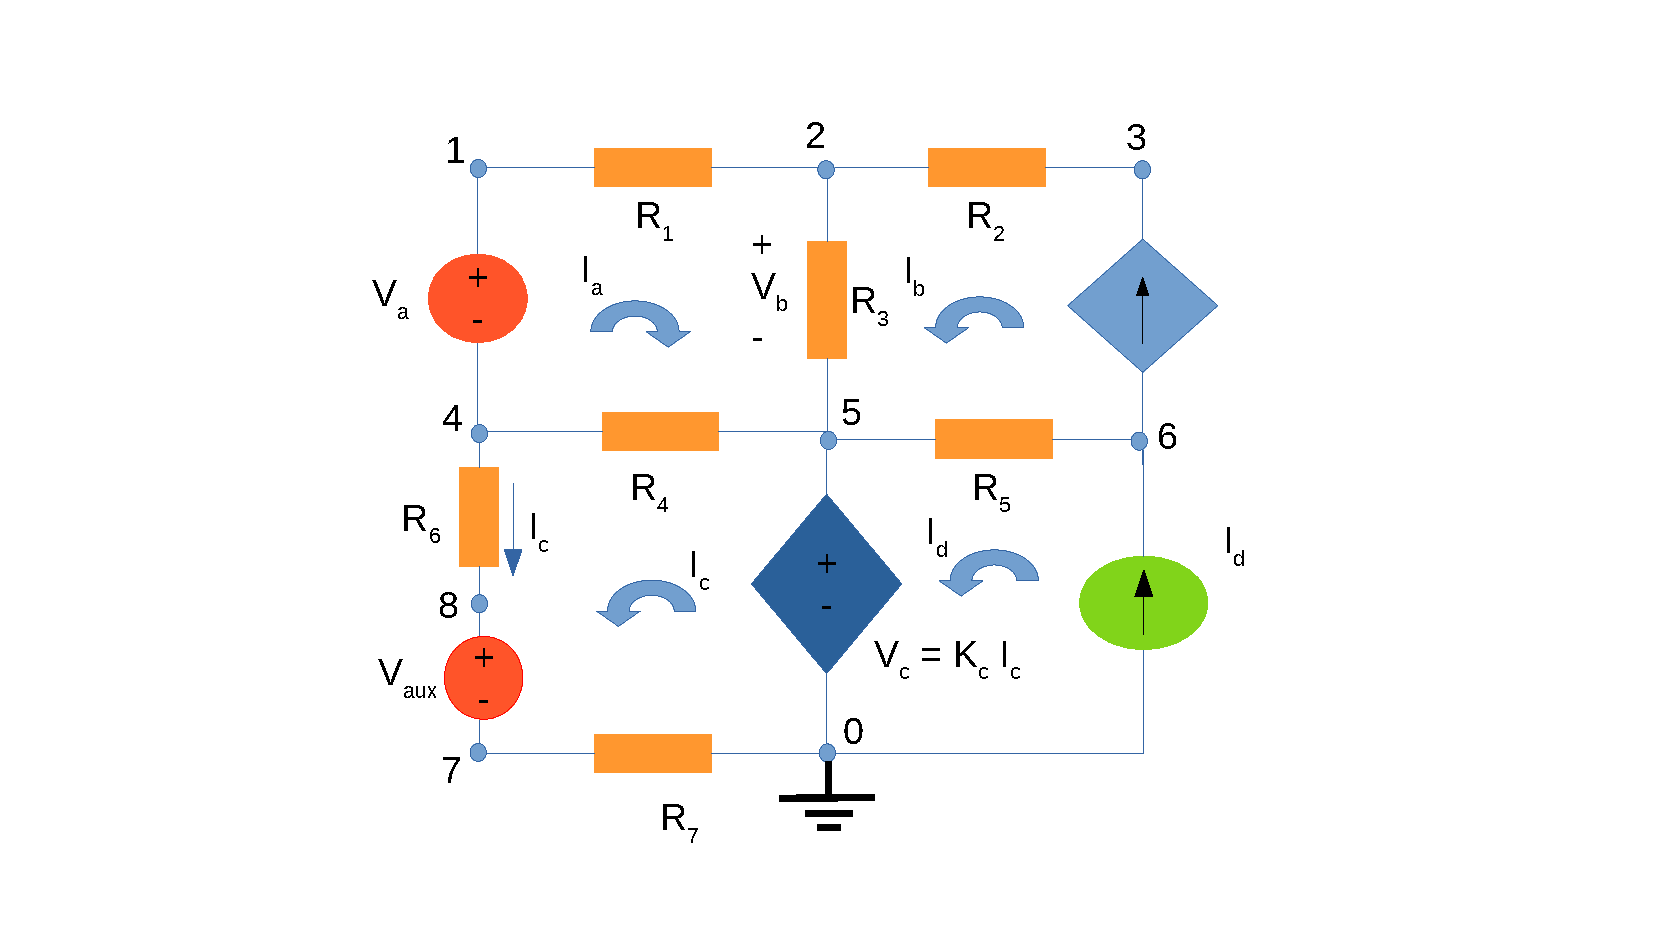
\includegraphics[width = 15cm]{system1.pdf}
\caption {Circuit}
\end{figure}





	The results obtained from the simulation are shown in the table below. 

\begin{table}[ht] \centering
\begin{tabular}{|
>{\columncolor[HTML]{FFCC67}}l l
>{\columncolor[HTML]{FFCC67}}l l|}
\hline
\cellcolor[HTML]{EABD8B}Name & \cellcolor[HTML]{EABD8B}Value {[}A or V{]} & \cellcolor[HTML]{EABD8B}Name & \cellcolor[HTML]{EABD8B}Value {[}A or V{]} \\ \hline
@Ib                          & -2.86455e-04                               & V1                           & 8.194795                                   \\
@Id                          & 1.029587e-03                               & V2                           & 7.917828                                   \\
@R1{[}i{]}                   & 2.732478e-04                               & V3                           & 7.340169                                   \\
@R2{[}i{]}                   & -2.86455e-04                               & V4                           & 2.978754                                   \\
@R3{[}i{]}                   & -1.32073e-05                               & V5                           & 7.957540                                   \\
@R4{[}i{]}                   & 1.229564e-03                               & V6                           & 1.197664e+01                               \\
@R5{[}i{]}                   & 1.316042e-03                               & V7                           & \cellcolor[HTML]{FFFFFF}9.776608e-01       \\
@R6{[}i{]}                   & 9.563162e-04                               & V8                           & 9.776608e-01                               \\
@R7{[}i{]}                   & 9.563162e-04                               & Vc                           & \cellcolor[HTML]{FFFFFF}7.327105e-05       \\
Vaux                         & 9.563162e-04                               & Va                           & -2.73248e-04                               \\ \hline
\end{tabular}
\caption{NgSpice simulation results}
\end{table}



	Then, an analysis of the values obtained was conducted, in order to ascertain the compatibility with the expected values from the theorethical analysis. This result validation was achieved by calculating the relative errors between the theoretical values obtained in octave and the experimental values obtained in ngspice.

\begin{table}[ht] \centering
\begin{tabular}{|
>{\columncolor[HTML]{FFCC67}}l |c|}
\hline
\multicolumn{2}{|l|}{\cellcolor[HTML]{EABD8B}Relative Errors (\%)} \\ \hline
{\color[HTML]{333333} V1}               & 0               \\ \hline
{\color[HTML]{333333} V2}               & 0               \\ \hline
{\color[HTML]{333333} V3}               & 0               \\ \hline
{\color[HTML]{333333} V4}               & 0               \\ \hline
{\color[HTML]{333333} V5}               & 0                       \\ \hline
{\color[HTML]{333333} V6}               & 0                       \\ \hline
{\color[HTML]{333333} V7}               & 0               \\ \hline
{\color[HTML]{333333} IA}               & 0              \\ \hline
{\color[HTML]{333333} IB}               & 3.49095e-05              \\ \hline
{\color[HTML]{333333} IC}               & 0                       \\ \hline
\end{tabular}
\caption{Relative Errors between Octave and NgSpice results}
\end{table}



	After the analysis of these errors, it is possible to infer that the accuracy is extremely high. The maximum relative error is 3.49095e-05, which is extremely low. This error is associated to the dissipated power in the resistors. Based on this, it is possible to conclude that the simulation results are validated.
